
\chapter{Paramagnetismo de Langevin y magnetismo de moléculas y compuestos químicos} % Main chapter title

\begin{center}

Hay \\
Un magnetismo mental \\
Entre nosotros, \\
Que nos delata \\
A kilómetros de distancias. . . \\
Y usted lo sabe

\hspace{3.6cm} Marco Valerio\\

\end{center}


\section{Paramagnetismo de Langevin}

Es adecuado suponer a los átomos paramagnético como pequeños imanes, a veces, llamados agujas magnéticas, esta imagen es adecuado para describir el comportamiento de los átomos paramagnéticos a altas temperaturas, para lo cual debemos suponer que no existe ningún tipo de interacción entre ellos. Langevin fue el primero que formuló una teoría sobre el paramagnetismo. Trata a la sustancia como un conjunto clásico de dipolos magnéticos sin interacciones, con un tratamiento similar al problema de encontrar el momento dipolar eléctrico en un dieléctrico en presencia de un campo eléctrico. Sin campo magnético externo los dipolos están desordenados al azar; no existiendo un momento magnético neto. La introducción del campo magnético externo genera una inhomogeneidad en el espacio e introduce una fuerza ordenadora capaz de orientar los dipolos magnéticos. Como consecuencia aparece una magnetización resultante. Cuando desparece el campo externo la agitación térmica genera el estado inicial nuevamente, (ya que supusimos que no hay ningún tipo de interacción entre los dipolos magnéticos). Dicho de otro modo es una competencia entre la fuerza ordenadora, magnética y la acción desordenadora de la temperatura. De aquí inferimos que la magnetización depende de la temperatura. La idea es hallar el momento magnético resultante del material al introducir el campo.


\subsection{Energía del dipolo}

La energía de un dipolo magnético en un campo, cuyo vector inducción es $B$ está dada por, donde observamos que el valor mínimo de la energía se obtiene cuando $\theta=0$ razón por lo cual se orientan los dipolos.

\begin{equation}
	E_{\mu}=-\V{\mu}\cdot\V{B} -\lv{\mu}\lv{B}Cos(\theta) =-\mu_{0}\;\mu\;H\;Cos(\theta)
\end{equation}

Sumando las proyecciones, en la dirección del campo, de todos los momentos magnéticos de los átomos o moléculas obtendríamos el momento magnético total de la sustancia. Es razonable suponer que no todos los átomos reaccionaran de igual manera, luego estamos en presencia de un problema estadístico, con un gran numero de partículas (átomos). El momento magnético resultante será un equilibrio estadístico entre la acción orientadora del campo externo y la desorientadora debido al movimiento térmico. El valor medio de las proyecciones de los momentos magnéticos individuales será la magnetización

\begin{equation}
	M=\left\langle \mu\;Cos(\theta) \right\rangle =\mu \left\langle Cos(\theta) \right\rangle
\end{equation}

Donde $N$ es el número de partículas por unidad de volumen, resta encontrar $\left\langle Cos(\theta) \right\rangle$ por ser un problema clásico podemos utilizar la distribución de Boltzmann que nos da la probabilidad de que el momento magnético este en un ángulo comprendido entre $\theta$ y $\theta + d\theta$ o lo que es equivalente dentro del ángulo sólido $\Omega$ como se observa en la figura. El ángulo sólido esta delimitado por la intercepción de dos conos sobre la esfera de radio $r$. El área de este sector es la longitud de la circunferencia cuyo radio es $2\pi r Sin(\theta)$ por la altura del sector $rd\theta$ o sea:

\begin{equation*}
	dS=2\pi r^{2}Sin(\theta)d\theta \quad \text{luego, tomando $r=1$ nos queda: } dS=2\pi Sin(\theta)d\theta = d\Omega
\end{equation*}

\begin{figure}[H]
    \centering
    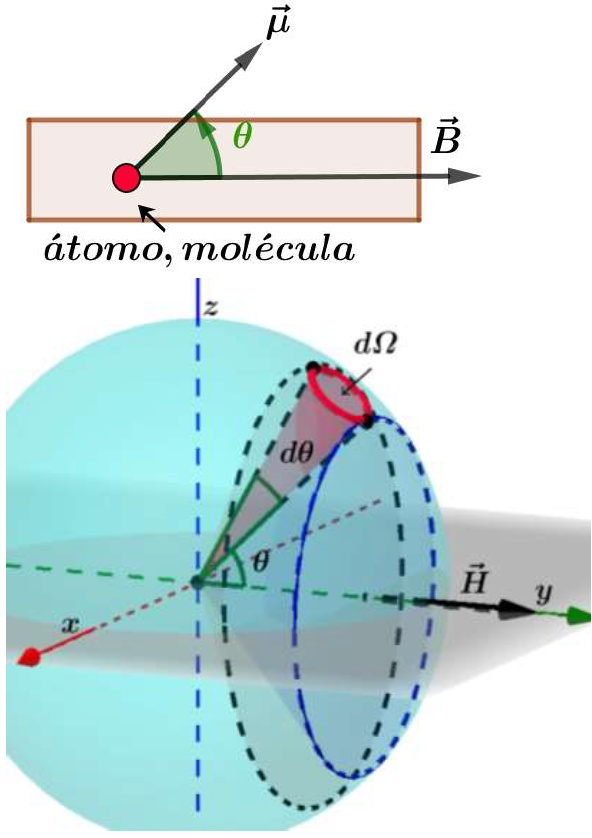
\includegraphics[width=0.6\textwidth]{./Figures/fig_c1}
	\caption{Momento magnético}
	\label{fig:c1}
\end{figure}

la probabilidad de una orientación para una dada energía es, 

\begin{equation}
	P(E)= \dfrac{\Bb{1}}{A'\;exp\left( \frac{E}{kT}\right) }
\end{equation}


donde $T$ es la temperatura en grados Kelvin, $k$ la constante de Boltzmann y $A'$ es una constante de normalización. No hay restricción sobre el número de partículas que pueden ocupar un dado estado Esta distribución es para partículas idénticas pero distinguibles. Luego:

\begin{equation}
	P(E)= A'\;exp\left( -\frac{E}{kT}\right) = A'\;exp\left( -\frac{\mu\mu_{0}\;N\;H\;Cos(\theta)}{kT}\right) = Ae^{\beta Cos(\theta)}
\end{equation}

Con $\Bb{\beta} =\left( -\frac{\mu\mu_{0}\;N\;H}{kT}\right)$ luego el valor medio será:

\begin{equation}
	M=\mu\langle Cos (\theta) \rangle= \mu \dfrac{\int Cos(\theta)exp(\beta Cos(\theta))d\Omega}{\int exp(\beta Cos(\theta))d\Omega}
\end{equation}

Extendida a todos los ángulos sólidos

\begin{equation}
\begin{aligned}
	M &= \mu \dfrac{\int_{0}^{2\pi} 2\pi Cos(\theta)exp(\beta Cos(\theta)) Sin(\theta)d\theta}{\int_{0}^{2\pi} 2\pi exp(\beta Cos(\theta)) Sin(\theta)d\theta}\\
	&= \mu \dfrac{\int_{0}^{2\pi} Cos(\theta)exp(\beta Cos(\theta)) d(Sin(\theta))}{\int_{0}^{2\pi} exp(\beta Cos(\theta)) d(Sin(\theta))}	\\
	&=
\mu \dfrac{\int_{-1}^{1} u\; exp(\beta u) du}{\int_{-1}^{1} exp(\beta u) du}	= \mu\dfrac{d}{d\beta}\left[ ln \left( \int_{-1}^{1} exp(\beta u) du \right)  \right] \\
	&= \mu \left[ \dfrac{e^{\beta}+e^{-\beta}}{e^{\beta}-e^{-\beta}}-\dfrac{1}{\beta} \right] \\
	&= \mu\left[ coth(\beta)-\dfrac{1}{\beta} \right] 
\end{aligned}
\end{equation}

La última expresión entre corchetes es llamada $L(\beta)$ función de Langevin.

Para valores pequeños de $\Bb{\beta} =\left( -\frac{\mu\mu_{0}\;N\;H}{kT}\right)$, o sea para $\mu\mu_{0}H < kT$ pequeños campos y temperaturas elevadas, podemos desarrollar la $Coth(\beta)= \dfrac{1}{\beta}+\dfrac{\beta}{3}+\dfrac{\beta^{3}}{45}+ \cdots$, luego si nos quedamos
con los dos primeros términos queda:

\begin{equation}
	M=\mu\langle Cos (\theta) \rangle= \mu \left[ Coth(\beta)-\dfrac{1}{\beta} \right] = \mu\dfrac{\beta}{3} = \dfrac{\mu^{2}\mu_{0}N}{3kT}
\end{equation}

luego la susceptibilidad paramagnética será

\begin{equation}
	\chi_{p} = \dfrac{M}{H} = \dfrac{\mu^{2}\mu_{0}N}{3kT}
\end{equation}

Esta expresión concuerda con la ley experimental llamada de Curie que nos indica que $\chi_{p}=\dfrac{c}{T}$

\begin{equation*}
\text{Langevin aplica} \rightarrow
				\begin{cases}
  				\text{Bien en: vapores y gases paramagneticos} \\
 				\text{Bien en: sales y metales a altas temperaturas} \\
  				\text{Mal en: metales paramagnetico sólidos}
    			\end{cases}
\end{equation*}

Es razonable pensar que los resultados en los sólidos metálicos no sean adecuados, puesto que unas de las premisas supuestas es que no existía interacción entre las partículas, cosa que evidentemente no es así. La suposición de un gas sin interacción entre partículas deja de ser valida. Pero, si la temperatura es elevada, la energía de las partículas supera a la de interacción entre ellas y modelo de gas es valido.

En la figura \ref{fig:c2} se observa representada la función de Langevin y la recta que se le aproxima para pequeños valores de $\beta$ La zona rayada indica su límite. Las deducciones anteriores se realizaron para la región donde rige la aproximación $\mu\mu_{0}H < kT$. Si contrariamente nos ubicamos donde vale $\mu\mu_{0}H >> kT$ entonces, $\beta\rightarrow\infty$ o sea, un valor muy grande, entonces, la ecuación

\begin{equation*}
	M= \mu \left[ Coth(\beta)-\dfrac{1}{\beta} \right] \approx \mu
\end{equation*}

Por tanto a temperaturas muy bajas la susceptibilidad paramagnética disminuye a medida que aumenta el campo. 

\begin{equation}
	\chi_{p} = \dfrac{M}{H} \approx \dfrac{\mu}{H}\rightarrow 0
\end{equation}


Con el objeto de contemplar la interacción atómica existente en los solidos metálicos, Weiss introdujo la idea de que a consecuencia de la interacción entre los momentos magnéticos se genera un muevo campo interno. O sea los átomos individuales interactuaban entre sí a través de un campo interno Weiss lo llamó \textbf{campo molecular} y lo supuso igual a: $\alpha M$.


\begin{figure}[H]
    \centering
    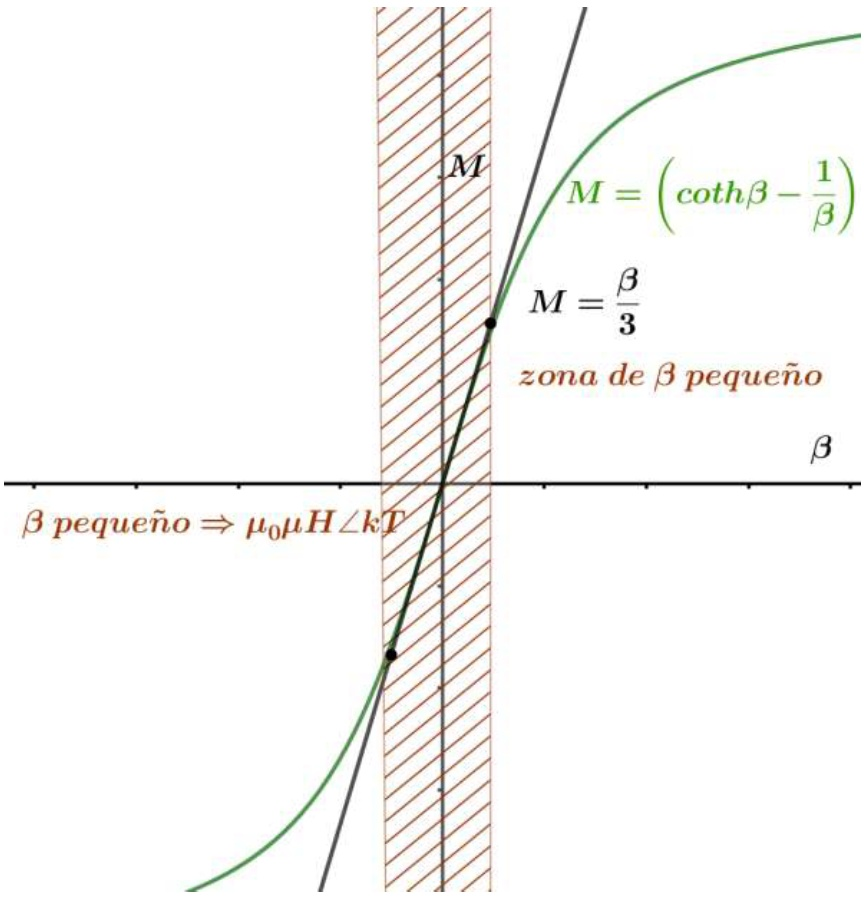
\includegraphics[width=0.6\textwidth]{./Figures/fig_c2}
	\caption{Función de Langevin}
	\label{fig:c2}
\end{figure}

Luego, si al campo externo $H$ le sumamos el interno, nos da el efectivo o total $H_{ef}=H+\alpha H$ si esta expresión la reemplazamos en:

\begin{equation}
\begin{aligned}
M &= \dfrac{\mu^{2}\mu_{0}N}{3kT}H =\dfrac{\mu^{2}\mu_{0}N}{3kT}(H+\alpha M) \\
  &= \dfrac{\mu^{2}\mu_{0}N}{3kT}H+ \alpha\dfrac{\mu^{2}\mu_{0}N}{3kT}M
  = M\left(1-\alpha\dfrac{\mu^{2}\mu_{0}N}{3kT} \right)
\end{aligned}
\end{equation}

Por lo que resulta que:

\begin{equation}
  \chi_{p}=\dfrac{M}{H}= \dfrac{\dfrac{\mu^{2}\mu_{0}N}{3kT}}{\left(1-\alpha\dfrac{\mu^{2}\mu_{0}N}{3kT} \right)}=\dfrac{\mu^{2}\mu_{0}N}{3k \left(T-\alpha\dfrac{\mu^{2}\mu_{0}N}{3k} \right)}= \dfrac{\alpha}{T-\theta}
\end{equation} 

Que es la ley de Curie Weiss donde $\alpha=\dfrac{\mu^{2}\mu N}{3k}$ y $\theta=\alpha^{2}$ llamada temperatura de Curie $T_{c}$ y marca el límite entre el estado paramagnético y ferromagnéticos del material. Este desarrollo muestra que un sólido paramagnético con momentos atómicos  localizados pero interactivos tendrá una susceptibilidad que obedece a la ley de Curie-Weiss.

\begin{figure}[H]
    \centering
    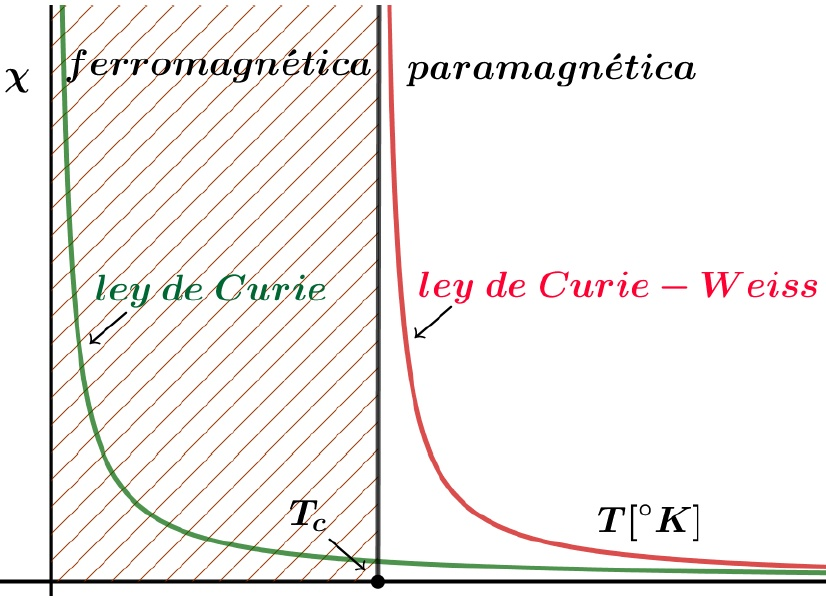
\includegraphics[width=0.6\textwidth]{./Figures/fig_c3}
	\caption{Ley de Curie-Wiess}
	\label{fig:c3}
\end{figure}

\section{Magnetismo de moléculas y compuestos químicos}

Hasta ahora conocemos tanto el origen del diamagnetismo como el del paramagnetismo. Podemos decir que átomos o iones podrían ser diamagnéticos o paramagnéticos. Vimos también un ejemplo de elementos paramagnéticos que dejan de serlo cuando se unen químicamente. Nos queda por estudiar el caso de moléculas y compuestos químicos. Si bien el caso del magnetismo de las moléculas o de compuestos es complejo podemos avanzar un poco más, pues nos servirá como introducción al ferromagnetismo.

\subsection{Teoría de los Orbitales Moleculares (TOM)}

La TOM es una metodología de mucha utilidad para determinar las propiedades magnéticas de moléculas y la estabilidad de las mismas. Sabemos que los átomos poseen orbitales donde la probabilidad de hallar electrones es máxima. La TOM supone también, que las moléculas poseen orbitales moleculares en donde se encuentran los electrones. Se asume que los electrones se mueven bajo la influencia de todos los núcleos que componen la molécula. Los orbitales moleculares se hallan como combinación lineal de los orbitales atómicos.

Si suponemos que la función de onda del orbital molecular es $\Psi$ y $\chi$ es la función de onda de los orbitales atómicos entonces:

\begin{equation}
	\Psi_{j} = \sum_{i=1}^{n}C_{ij}\chi_{i}
\end{equation}

Durante la formación de la molécula, él o los átomos y sus orbitales se acercan y comienzan a interactuar, formando los nuevos orbitales moleculares que pertenecen a la molécula en su totalidad y no a un solo átomo.

\subsection{Magnetismo de moléculas y compuestos químicos}

\begin{itemize}
	\item El numero de orbitales moleculares es igual al número de orbitales atómicos que se solapan. 		
	\item Para ir avanzando sobre el tema tomemos el ejemplo de una molécula formada por átomos iguales $H_{2}$ . En el esquema se observa los dos orbitales atómicos $1s$, que al interactuar formas los orbitales moleculares enlazante $\sigma_{1s}$ de menor energía que el antideslizante $\sigma_{1s}^{*}$ . Por supuesto, los niveles energéticos de los átomos de hidrógeno, antes de la reacción son iguales.
	
\begin{figure}[H]
    \centering
    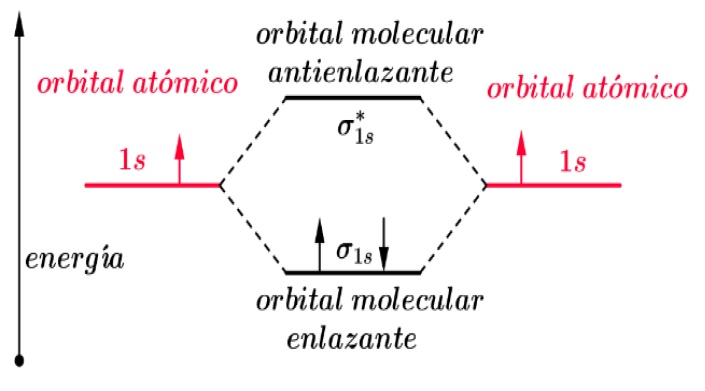
\includegraphics[width=0.6\textwidth]{./Figures/MagMolecular}
	\caption{Magnetismo Molecular}
	\label{fig:MagMolecular}
\end{figure}

Se llama orden de enlace ($OE$) al parámetro que indica la estabilidad de la unión. Se define como la mitad de la diferencia entre el número de electrones en los Orbitales enlazantes menos el número de electrones en los orbitales antienlazantes. Si el resultado es positivo la unión es estable

\begin{equation}
	OE=\frac{OE-OA}{2}=\frac{2-0}{2}=1
\end{equation}
	
	
	\item Si a la molécula $H_{2}$ la irradiamos con luz ultravioleta puede pasar un electrón al orbital antienlazante, absorbiendo energía con lo cual el $OE$ seria 0, luego la molécula deja de existir.
	
	\item Estudiemos el caso de una molécula de gas noble que no existe $He_{2}$ en este caso será:

En todos los casos se debe respetar el \textbf{Principio de Pauli}: recordemos que no puede haber dos electrones con todos sus números cuánticos iguales, en el mismo estado dentro del mismo sistema y el \textbf{Principio de Hund} que dice: Los electrones se ubican dentro de los orbitales de la misma energía de manera que estén desapareados al máximo

\begin{figure}[H]
    \centering
    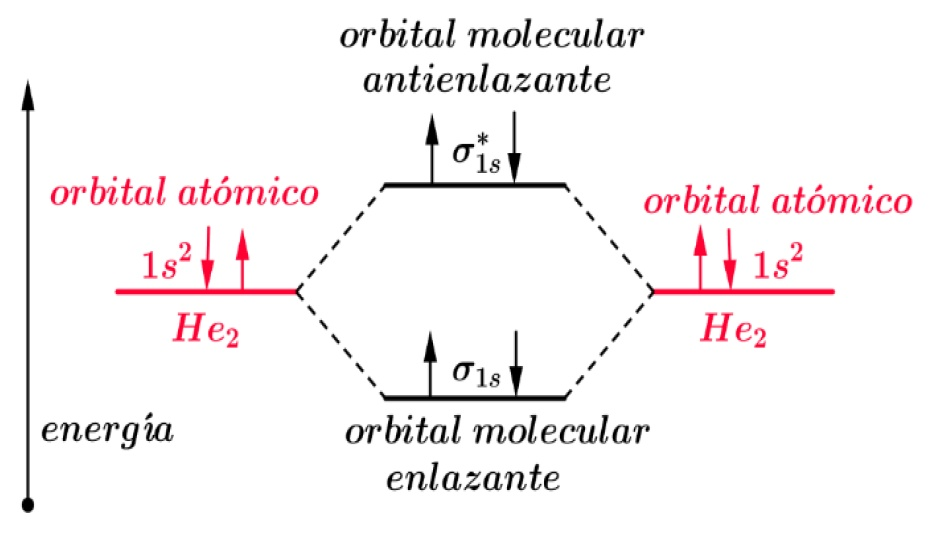
\includegraphics[width=0.6\textwidth]{./Figures/MagMolecularHe2}
	\caption{Magnetismo Molecular del $He_{2}$}
	\label{fig:MagMolecular}
\end{figure}

\begin{equation}
	OE=\frac{OE-OA}{2}=\frac{2-2}{2}=0
\end{equation}

Luego, la molécula no es estable.
\end{itemize}


\subsubsection{Casos en que entra en juego el segundo nivel energético}

En el caso que interactúen orbitales $2s$ el procedimiento es igual al caso anterior. En la figura, de abajo, se observa un esquema de los orbitales $s$, con n significamos el número cuántico principal, puesto que todos los $s$ serán Iguales.

\begin{figure}[H]
    \centering
    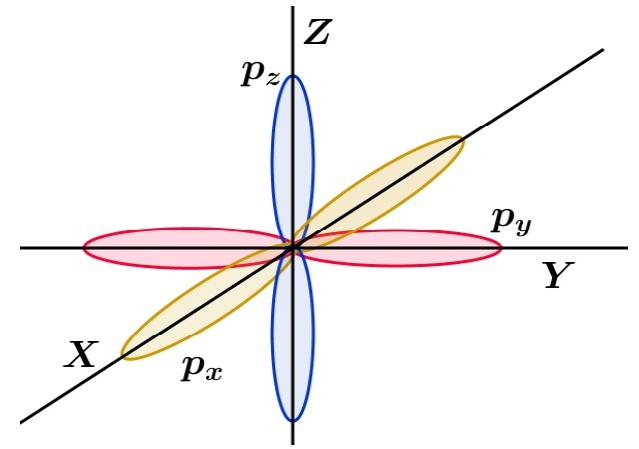
\includegraphics[width=0.6\textwidth]{./Figures/SegundoNivelEnergetico}
	\caption{Segundo nivel energético orbitales $s$}
	\label{fig:SegundoNivelEnergetico}
\end{figure}

Difiere un poco cuando trabajos con los orbitales $2p$, ya que, no son esféricos y se sitúan a lo largo de los tres ejes $x$, $y$, $z$ del espacio. Para entender un poco mejor como se unen los átomos seguiremos trabajando con los orbitales. A medida que los átomos se acercan comienzan a interactuar los orbitales atómicos y forman, por combinación lineal los orbitales moleculares. Se dan distintas posibilidades según que orbitales atómicos se enfrentan. Supongamos que enfrentamos dos órbita $2p_{x}$, como indica el esquema, esta interacción dará origen a dos orbitales moleculares.

\begin{figure}[H]
    \centering
    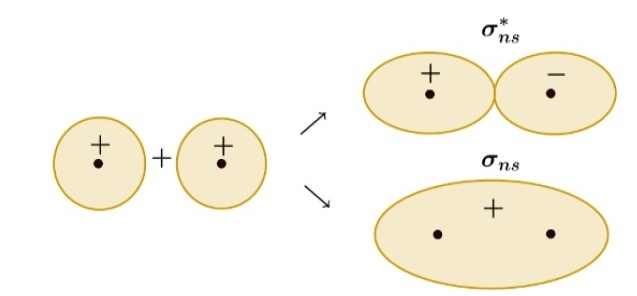
\includegraphics[width=0.7\textwidth]{./Figures/Molecula2doNivel1}
	\caption{Segundo nivel energético dos orbitales $s$}
	\label{fig:Molecula2doNivel1}
\end{figure}

En la figura \ref{fig:Molecula2doNivel2} se observa un esquema donde reaccionan dos orbitales atómicos enfrentado en la dirección $x$ mientras que en la figura \ref{fig:Molecula2doNivel3} los orbitales que reaccionan están en la dirección $y$.

\begin{figure}[H]
    \centering
    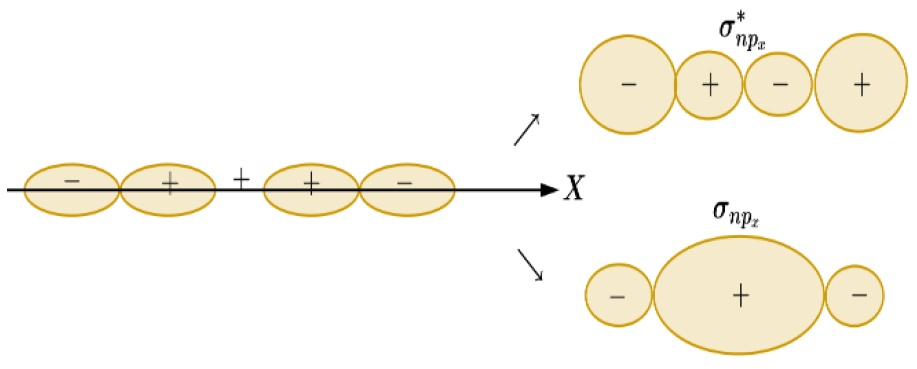
\includegraphics[width=0.7\textwidth]{./Figures/Molecula2doNivel2}
	\caption{Orbitales enfrentados en la dirección $x$}
	\label{fig:Molecula2doNivel2}
\end{figure}

\begin{figure}[H]
    \centering
    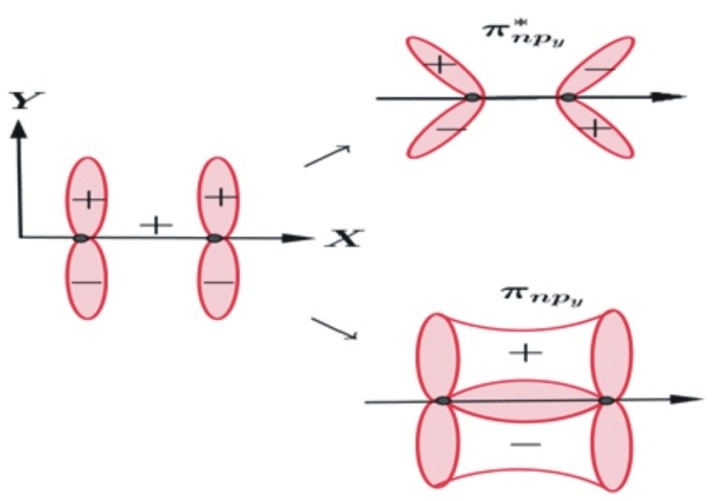
\includegraphics[width=0.7\textwidth]{./Figures/Molecula2doNivel3}
	\caption{Orbitales enfrentados e la dirección $y$}
	\label{fig:Molecula2doNivel3}
\end{figure}
	
	
Algo similar sucede si los orbitales paralelos estuviesen en la dirección z. En estos dos últimos casos los orbitales moleculares se designan con $\pi_{np_{y}}$ , $\pi_{np_{z}}$ o $\pi_{np_{y}}^{*}$ , $\pi_{np_{z}}^{*}$

\subsubsection{Ejemplo: molécula del $Ni_{2}$}

\begin{itemize}
	\item Comenzamos por la configuración electrónica del Nitrógeno ($Z=7$):
	\begin{equation}
		1s^{2}2s^{2}2p^{1}_{x}2p^{1}_{y}2p^{1}_{z}
	\end{equation}
	\item Los orbitales se llenan de acuerdo a las principios de \textbf{Pauli y Hund}. 
	\item Los orbitales atómicos tienen las mismas energía, por eso se encuentran al mismo nivel. No pasaría lo mismo si los átomos son distintos.
	\item Los orbitales moleculares de menor enegía se llenan primero.
	\item En este caso los orbitales enfrentados son los $2p_{z}$
	\item \textbf{Esta molécula es diamagnética, puesto que tiene los electrones apareados, los átomos son paramagnéticos}
	\item Si los átomo que reaccionan tiene pocos electrones, no solo hay interacción $s-s$ y $p-p$ sino que aparece otra interacción $s-p$ que modifica los niveles de los orbitales moleculares esto se observa en el esquema de la figura \ref{fig:EjemploNi2}.
\end{itemize}

\begin{figure}[H]
    \centering
    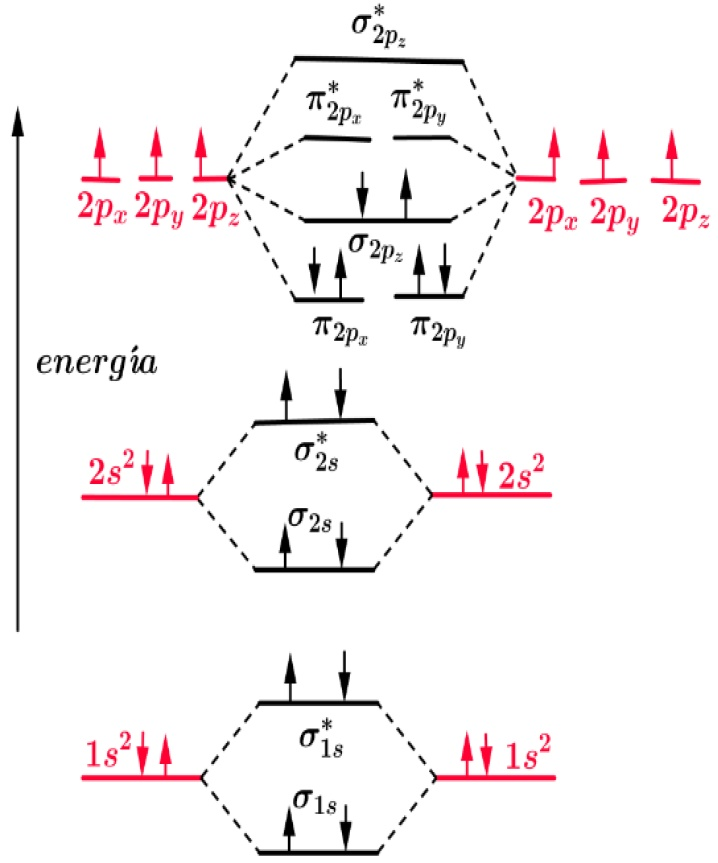
\includegraphics[width=0.6\textwidth]{./Figures/EjemploNi2}
	\caption{Molécula de $Ni_{2}$}
	\label{fig:EjemploNi2}
\end{figure}

\newpage

\subsubsection{Interacción cruzada}

\textbf{Para átomos con $N \leq 7 $ electrones}

\begin{figure}[H]
    \centering
    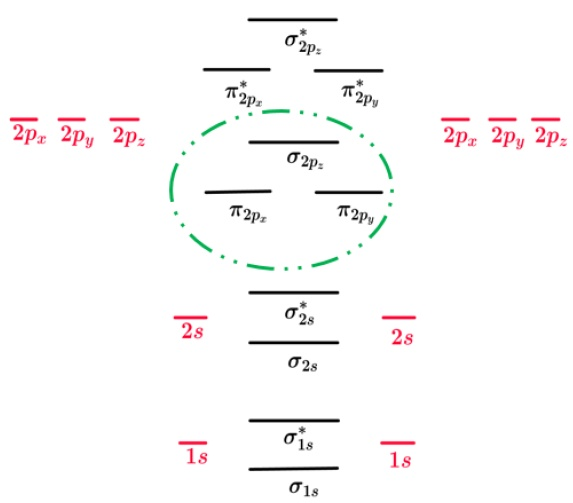
\includegraphics[width=0.7\textwidth]{./Figures/interaccionCruzada7a}
	\caption{Interacción cruzada $N \leq 7$}
	\label{fig:interaccionCruzada7a}
\end{figure}


\textbf{Para átomos con $N>7$ electrones}

\begin{figure}[H]
    \centering
    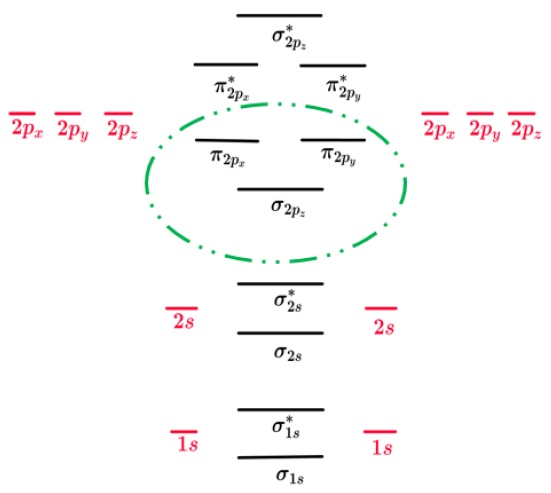
\includegraphics[width=0.7\textwidth]{./Figures/interaccionCruzada7b}
	\caption{Interacción cruzada $N > 7$}
	\label{fig:interaccionCruzada7b}
\end{figure}


\newpage
\subsubsection{Caso del Oxígeno $Z=8$}


\textbf{$O_{2}$ - Paramagnético:}

\begin{figure}[H]
    \centering
    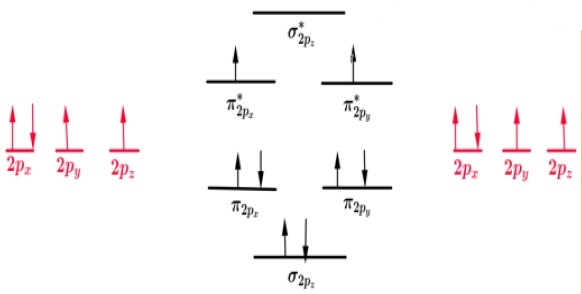
\includegraphics[width=0.7\textwidth]{./Figures/interaccionCruzadaOxigenoA}
	\caption{$O_{2}$ Paramagnético}
	\label{fig:interaccionCruzadaOxigenoA}
\end{figure}

\textbf{$O_{2}^{+}$ - Paramagnético:}

\begin{figure}[H]
    \centering
    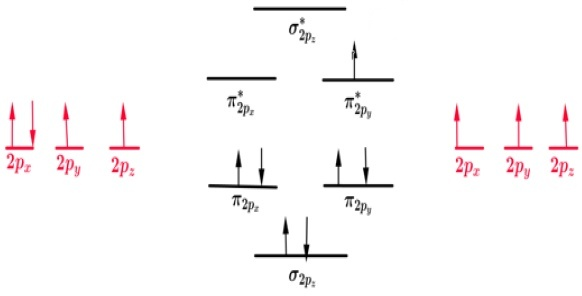
\includegraphics[width=0.7\textwidth]{./Figures/interaccionCruzadaOxigenoC}
	\caption{$O_{2}^{+}$ Paramagnético}
	\label{fig:interaccionCruzadaOxigenoC}
\end{figure}


\textbf{$O_{2}^{2+}$ - Diamagnético:}

\begin{figure}[H]
    \centering
    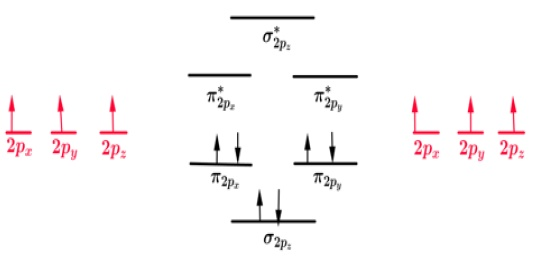
\includegraphics[width=0.7\textwidth]{./Figures/interaccionCruzadaOxigenoB}
	\caption{$O_{2}^{2+}$ Diamagnético}
	\label{fig:interaccionCruzadaOxigenoB}
\end{figure}


\textbf{$O_{2}^{2-}$ - Diamagnético:}

\begin{figure}[H]
    \centering
    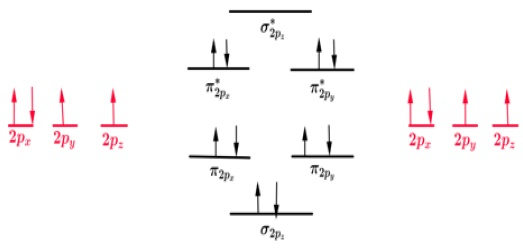
\includegraphics[width=0.6\textwidth]{./Figures/interaccionCruzadaOxigenoD}
	\caption{$O_{2}^{2-}$ Diamagnético}
	\label{fig:interaccionCruzadaOxigenoD}
\end{figure}

\subsubsection{Compuestos de átomos distintos}

Hasta ahora hemos visto moléculas di atómicas de átomos iguales, nos está faltando el magnetismo de moléculas formadas por átomos distintos. En este caso la dificultad está en que al no ser átomos iguales, estos no tienen los mismos niveles de energía. Tengamos presente que los átomos más electronegativos tienen menor energía.

Los orbitales moleculares se llenan como hasta ahora teniendo en cuenta los principios de Pauli y Hund.

Veamos dos casos clásicos $CO$ y $NO$.

\textbf{Para el CO:}

Se debe comenzar con la configuración electrónica de cada elemento
\begin{equation}
\begin{aligned}
	C: He+ 2s^{2}2p^{2} \\
	O: He+ 2s^{2}2p^{4}
\end{aligned}
\end{equation}

No se dibujan los niveles $1s^{2}$ por ser iguales en todos los casos.
Los niveles moleculares se observan en la figura \ref{fig:CO2Diamagnetico}:

\begin{figure}[H]
    \centering
    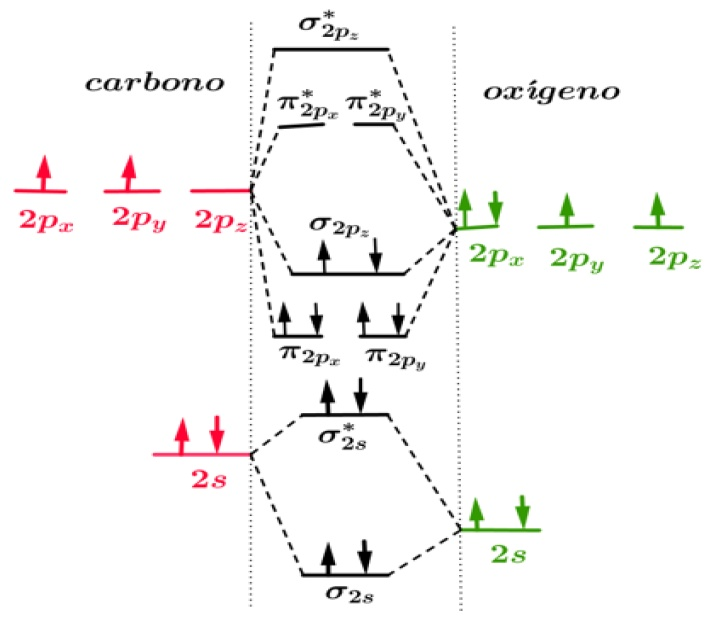
\includegraphics[width=0.6\textwidth]{./Figures/CO2Diamagnetico}
	\caption{$CO_{2}$ Diamagnético}
	\label{fig:CO2Diamagnetico}
\end{figure}


\textbf{Para el NO:}

La configuración electrónica del nitrógeno es
\begin{equation}
	N: He+ 2s^{2}3p^{3}
\end{equation}
No dibujamos el vector que Indica la dirección en la que aumenta la energía pues es similar al caso anterior.
Por tener un electrón desapareado esta molécula es paramagnética.

\begin{figure}[H]
    \centering
    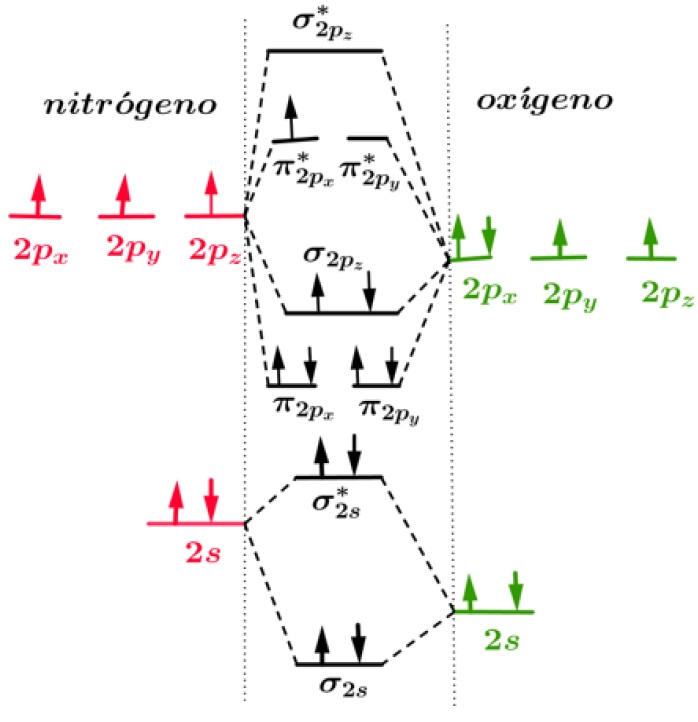
\includegraphics[width=0.6\textwidth]{./Figures/CO2Paramagnetico}
	\caption{$CO_{2}$ Paramagnético}
	\label{fig:CO2Paramagnetico}
\end{figure}

Tengamos presente que:

\begin{itemize}
	\item Todas las moléculas formadas por átomos distintos presentan esquemas de energía similares.
	\item Estamos comentando solo los casos más simples, existen moléculas donde la complicación es mayor.
	\item En todos estos casos se podría haber calculado el orden de enlace.
\end{itemize}

